% One Britannica scan as extracted by Nemotron Parse 3.5. Filled by src/nemotron_challenge/stages/latex.py.
% The TITLE, BODY and SOURCE markers (each wrapped in two percent signs) are replaced. Compile with XeTeX (tectonic).
\documentclass[10pt]{article}
\usepackage[a4paper,margin=18mm]{geometry}
\usepackage{fontspec}
\usepackage{multicol}
\usepackage{graphicx}
\usepackage[hidelinks]{hyperref}
\usepackage[normalem]{ulem}
\setlength{\parindent}{0pt}
\setlength{\parskip}{4pt}
\setlength{\columnsep}{8mm}
\begin{document}
\section*{Historical source: MAGNETISM}
\begin{multicols}{2}
\subsection*{\textit{continued:} MAGNETISM}
{\small\itshape [Margin: 41 tempered sheet from a the magma film.]}\par
But any degree of temper that is given to \sout{feed} \textbf{steel} makes a very important change in this respect. In the first place, it acquires \sout{magnentifin} \textbf{magnetism} more \sout{flowly} \textbf{slowly} by induction than an equal and similar piece of common iron, and \sout{its maly acquired lets.} \textbf{finally acquires left.} These differences are \sout{only transmined} \textbf{easily examined} by the deviations which it causes in the \sout{manner’s} \textbf{mariner's} needle from the magnetic meridian, and by its \sout{attractive tions.} \textbf{attraction.} When the inducing magnet is removed, fome \sout{magnetti} \textbf{magnetism} remains in the fixed bar, which retains the \sout{polory which,} \textbf{polarity which} it \sout{will be} \textbf{had in} the \sout{neighborhood} \textbf{neighbourhood} of the \sout{matter.} \textbf{magnet.} Steel tempered to the degree fit for watch Springs acquires \sout{along magnetic} \textbf{a strong magnetism} which \sout{is} \textbf{it} exhibits \sout{imme disels} \textbf{immediately} on the removal of the magnet. But it diffipates very \sout{fat ;} \textbf{fast;} and, in a very few minutes, it is reduced to \sout{lois} \textbf{less} than one half of its strength while in \sout{control} \textbf{contact} with the magnet, and not two thirds of what it was \sout{distety} \textbf{immediately} on removal from it. It continues to \sout{diffidate} \textbf{diffipate} for former days, though the \sout{her} \textbf{bar} be kept with \sout{care';} \textbf{care;} but the diffusion diminishes at, and in the near at, half over third of its greatest power \sout{forany} \textbf{for any} length of time, \sout{unleef cardially keep} \textbf{unless carefully kept} or \sout{indjudicially} \textbf{injudiciously} treated. Steel tempered \sout{into flowing} \textbf{for strong} cutting tools, \sout{fish a schlieb,} \textbf{fuch as chifels,} punches, and drills for metal, acquires \sout{magnifin} \textbf{magnetifm} fill more flowly by induction, and acquires \sout{five} \textbf{lefs} of it while in \sout{contact} \textbf{conta\&} with the \sout{magnet,} \textbf{magnet;} but it \sout{certain} \textbf{retains} it more \sout{firms by,} \textbf{firmly,} and finally retains a greater proportion of \sout{who} \textbf{what} it had acquired. Steel made as hard as \sout{possible,} \textbf{poffible,} is much longer in \sout{acquiring} \textbf{ac-quiring} all the \sout{magnifin} \textbf{magnifim} which limple \sout{juxtaposition} \textbf{juxtapofition} can give to it. It acquires \sout{less} \textbf{lefs} than the \sout{formerly} \textbf{former;} but it retains \sout{is} \textbf{it} with great \sout{firmness,} \textbf{firmnefs,} and finally retains a much greater proportion. Such one of iron as are fulcypible of magnetifi, are nearly like hard feel in their effects you that in the time necessary for their \_properlift\_ impregnation, and in the durability of the acquired magnifine. They effic exceedingly in respect to the degree of power which they can attain by mere juxtaption, and the virieties form to depend on heterogeneous mixture. We emit offriever, thus far once of our ones of influence of of magnetism of the metal in the fate of my way, and \sout{combred} \textbf{com-bred} with dolphins, are not magnentable while remaining in that there. Mott core require reading, and a fort of cementation, in contact with inflammable fuhlances. This matter is not underdefended, but it would form that complex metallization is far from being the north to votrale condition, and that a certain degree of \sout{oxydation,} \textbf{oxyda-tion,} and perhaps some other positive yet unknown, make the her lautiness. Our all this is extremely oblicure. The late Dr Cowin Knight made a \sout{compoliotion} \textbf{compolio-tion} which required every phono and permanent \sout{magseting,} \textbf{mag-seting,} but the recent died with him. Dr Gilbert peaks of limilat compositions, in which ferruginous days were ingredients ; but we know nothing of the fate of the metal in them, nor their mode of acquiring \sout{magretin.} \textbf{mag-retin.} It is of peculiar importance to \sout{work} \textbf{remark} that the \sout{acquition} \textbf{acquisition} of \sout{magnetization} \textbf{magnetism} is gradual and \sout{progrestive,} \textbf{progressive,} and that the gradation is the more perceptible in proportion as the field is of a \sout{hastheric} \textbf{harder} temper. When a magnet is \sout{hrough} \textbf{brought} to one end of a bar of common iron, \sout{to} \textbf{its} remote extremity, \sout{unleef} \textbf{unless} exceedingly long, \sout{requires} \textbf{acquires} its utmost \sout{magnifin} \textbf{magnetism} immediately. But when the north pole of Surez, Vol. II. Part I. a magnet is applied: to one end of a bar of hard flee, the part in contact immediately becomes a fourth pole, and the far end is not yet affected. We offer a north pole formed a fance difference from the concept, and \sout{becsent} \textbf{bec-sent} that a faint tooth pole. \sout{"Their} \textbf{Their} gradually advance along the bar. The remote extremity become frit a faint fourth pole, and it is not differ very long while (If ceer) that it becomes a simple, vigorous, north pole. More frequently it remains a difficult and recycle north pole: may, if the her for very long, it often \sout{hoppus} \textbf{hop-pus} that have a sacrifice of north and forth poles, which never make their way to the far end of the bar. This phenomenon was first observed (we think) by Dr Brook Taylor, who \_they\_ now account of his obtivations to the \_Philophysical Transformation\_, no 344. From the account we have given of their \sout{phenomenons} \textbf{phenomena} to a stof indeed magnifine, it appears that the temporary because magnifin is always lo disfpided that the rim of their beces mutual attractions of the difficiliate poles exceeds the gentich im of the repollon between the \sout{limlar,} \textbf{limilar} poles, and that therefore the two magnets tend to each other. This is evidently equivalent to \sout{flying,} \textbf{faying,} that a piece of magnungtic iron is always attracted by a magnet. No exception has ever been \sout{observed} \textbf{oberved} to this fact, for Phys's dury of a Thamades, or loadlines, which repeals iron, is allowed by all to have been a false. We think \sout{outfellow authorified} \textbf{ourfelves authorifed} to \sout{lay} \textbf{fay} that this attraction of the \sout{headlines} \textbf{loadfione} for iron, or this tendency of iron to the \sout{headline,} \textbf{loadfione,} is a \sout{secondary} \textbf{fecondary} phenomenon, and is the \sout{\_conference\_} \textbf{confequence} of the proper \sout{disposition} \textbf{difpofition} of the induced \sout{magnetimin.} \textbf{magnetifm.} The proofs already given of the compound \sout{matters} \textbf{nature} of this \sout{phenomena,} \textbf{phenomenon,} namely, that \sout{is arise} \textbf{it arifes} from the excess of two \sout{attributions} \textbf{attractions} above two \sout{repetitions,} \textbf{repulsions,} need (we imagine) no addition. But the following \sout{condiractions} \textbf{confiderations} place the matter beyond doubt. I. The \sout{magnifinal} \textbf{magnetifm} of the two poles is evidently of an opposite nature; the one repelling what the other \sout{attrade).} \textbf{attracts.} If the \sout{aircraft} \textbf{one attracts} iron, therefore, the other should \sout{result} \textbf{repel} it. But each \sout{path,} \textbf{pole,} by \sout{changing} \textbf{inducing} a \sout{magretifion} \textbf{magnetifm} opposite to its own, on the nearest end of the iron, and the \sout{fans} \textbf{fame} with its own on the remote end, and its action diminishing with an increase of \sout{diflants,} \textbf{distance,} there \sout{mult} \textbf{must} always be an excess of attraction, and the iron \sout{mult} \textbf{must} be \sout{attached.} \textbf{attracted.} A Each of the magnets A and B, in either of the positions \sout{reprefened} \textbf{represented} in fig. 12. would alone attract the piece of common iron. But when placed together, the fourth pole of \sout{8} \textbf{B} tends to render the upper end of C a north pole; while the north pole of B tends to take it a South pole. If \sout{there} \textbf{their} actions be nearly equal, the weight of C cannot be \sout{supposedly be} \textbf{supported by} the \sout{magnifin} \textbf{magnetism} induced by any difference of action that may remain. While C is hanging \sout{D I} \textbf{by B} alone, \sout{let.} \textbf{let} A be gradually \sout{enough tree,} \textbf{brought near;} it gradually \sout{thorley} \textbf{destroys} the action of the north pole of B, \sout{to} \textbf{so} that C gradually \sout{lofos} \textbf{loses} its \sout{magnifin} \textbf{magnetism} and polarity, and its weight \sout{prends.} \textbf{prevails.} §. He all three cases where the induction of magnetifism is flow, the attraction is weak in proportion. This is particularly remarked by Dr Gilbers. If we take piece of common iron, and of fleet of different temps, but all of the fame fine and form, we shall find that the iron is much more thought attracted than any of the rel, and that the attraction for each of them a weaker proportion as they are harder. This liberty is to accurately observed, that when the piece is thoroughly

\begin{center}
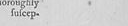
\includegraphics[width=\linewidth,height=0.4\textheight,keepaspectratio]{../crops/e0756-02.png}
\par{\small \textit{Plate:} R}
\end{center}
\end{multicols}
\section*{Source record}
\begin{itemize}
\item Page ID: \texttt{britannica:309f765b1ecc83e0a7f7762e44b4a927a7555443:train:756}
\item Scan: \texttt{page-0756-33eb91fcbe8d.jpg}, 600 x 810 px
\item Image SHA-256: \texttt{\small 33eb91fcbe8d9d080f38ca26a23b791f56382bebff38a428cd4ac3cd30fb48f3}
\item Extraction: \texttt{nvidia/nemotron-3.5-parse}, raw reply \texttt{artifacts/extract/raw/0756.json}
\item Text is Parse OCR output, normalized (long s as s, line-end hyphens joined). It is not corrected by hand.
\item \sout{Struck-through} words are Parse's reading; \textbf{bold} words are Super VL's correction, checked against the scan image. Both are model output.
\end{itemize}
\end{document}
